% Options for packages loaded elsewhere
\PassOptionsToPackage{unicode}{hyperref}
\PassOptionsToPackage{hyphens}{url}
%
\documentclass[
]{article}
\usepackage{amsmath,amssymb}
\usepackage{lmodern}
\usepackage{iftex}
\ifPDFTeX
  \usepackage[T1]{fontenc}
  \usepackage[utf8]{inputenc}
  \usepackage{textcomp} % provide euro and other symbols
\else % if luatex or xetex
  \usepackage{unicode-math}
  \defaultfontfeatures{Scale=MatchLowercase}
  \defaultfontfeatures[\rmfamily]{Ligatures=TeX,Scale=1}
\fi
% Use upquote if available, for straight quotes in verbatim environments
\IfFileExists{upquote.sty}{\usepackage{upquote}}{}
\IfFileExists{microtype.sty}{% use microtype if available
  \usepackage[]{microtype}
  \UseMicrotypeSet[protrusion]{basicmath} % disable protrusion for tt fonts
}{}
\makeatletter
\@ifundefined{KOMAClassName}{% if non-KOMA class
  \IfFileExists{parskip.sty}{%
    \usepackage{parskip}
  }{% else
    \setlength{\parindent}{0pt}
    \setlength{\parskip}{6pt plus 2pt minus 1pt}}
}{% if KOMA class
  \KOMAoptions{parskip=half}}
\makeatother
\usepackage{xcolor}
\usepackage[margin=1in]{geometry}
\usepackage{color}
\usepackage{fancyvrb}
\newcommand{\VerbBar}{|}
\newcommand{\VERB}{\Verb[commandchars=\\\{\}]}
\DefineVerbatimEnvironment{Highlighting}{Verbatim}{commandchars=\\\{\}}
% Add ',fontsize=\small' for more characters per line
\usepackage{framed}
\definecolor{shadecolor}{RGB}{248,248,248}
\newenvironment{Shaded}{\begin{snugshade}}{\end{snugshade}}
\newcommand{\AlertTok}[1]{\textcolor[rgb]{0.94,0.16,0.16}{#1}}
\newcommand{\AnnotationTok}[1]{\textcolor[rgb]{0.56,0.35,0.01}{\textbf{\textit{#1}}}}
\newcommand{\AttributeTok}[1]{\textcolor[rgb]{0.77,0.63,0.00}{#1}}
\newcommand{\BaseNTok}[1]{\textcolor[rgb]{0.00,0.00,0.81}{#1}}
\newcommand{\BuiltInTok}[1]{#1}
\newcommand{\CharTok}[1]{\textcolor[rgb]{0.31,0.60,0.02}{#1}}
\newcommand{\CommentTok}[1]{\textcolor[rgb]{0.56,0.35,0.01}{\textit{#1}}}
\newcommand{\CommentVarTok}[1]{\textcolor[rgb]{0.56,0.35,0.01}{\textbf{\textit{#1}}}}
\newcommand{\ConstantTok}[1]{\textcolor[rgb]{0.00,0.00,0.00}{#1}}
\newcommand{\ControlFlowTok}[1]{\textcolor[rgb]{0.13,0.29,0.53}{\textbf{#1}}}
\newcommand{\DataTypeTok}[1]{\textcolor[rgb]{0.13,0.29,0.53}{#1}}
\newcommand{\DecValTok}[1]{\textcolor[rgb]{0.00,0.00,0.81}{#1}}
\newcommand{\DocumentationTok}[1]{\textcolor[rgb]{0.56,0.35,0.01}{\textbf{\textit{#1}}}}
\newcommand{\ErrorTok}[1]{\textcolor[rgb]{0.64,0.00,0.00}{\textbf{#1}}}
\newcommand{\ExtensionTok}[1]{#1}
\newcommand{\FloatTok}[1]{\textcolor[rgb]{0.00,0.00,0.81}{#1}}
\newcommand{\FunctionTok}[1]{\textcolor[rgb]{0.00,0.00,0.00}{#1}}
\newcommand{\ImportTok}[1]{#1}
\newcommand{\InformationTok}[1]{\textcolor[rgb]{0.56,0.35,0.01}{\textbf{\textit{#1}}}}
\newcommand{\KeywordTok}[1]{\textcolor[rgb]{0.13,0.29,0.53}{\textbf{#1}}}
\newcommand{\NormalTok}[1]{#1}
\newcommand{\OperatorTok}[1]{\textcolor[rgb]{0.81,0.36,0.00}{\textbf{#1}}}
\newcommand{\OtherTok}[1]{\textcolor[rgb]{0.56,0.35,0.01}{#1}}
\newcommand{\PreprocessorTok}[1]{\textcolor[rgb]{0.56,0.35,0.01}{\textit{#1}}}
\newcommand{\RegionMarkerTok}[1]{#1}
\newcommand{\SpecialCharTok}[1]{\textcolor[rgb]{0.00,0.00,0.00}{#1}}
\newcommand{\SpecialStringTok}[1]{\textcolor[rgb]{0.31,0.60,0.02}{#1}}
\newcommand{\StringTok}[1]{\textcolor[rgb]{0.31,0.60,0.02}{#1}}
\newcommand{\VariableTok}[1]{\textcolor[rgb]{0.00,0.00,0.00}{#1}}
\newcommand{\VerbatimStringTok}[1]{\textcolor[rgb]{0.31,0.60,0.02}{#1}}
\newcommand{\WarningTok}[1]{\textcolor[rgb]{0.56,0.35,0.01}{\textbf{\textit{#1}}}}
\usepackage{longtable,booktabs,array}
\usepackage{calc} % for calculating minipage widths
% Correct order of tables after \paragraph or \subparagraph
\usepackage{etoolbox}
\makeatletter
\patchcmd\longtable{\par}{\if@noskipsec\mbox{}\fi\par}{}{}
\makeatother
% Allow footnotes in longtable head/foot
\IfFileExists{footnotehyper.sty}{\usepackage{footnotehyper}}{\usepackage{footnote}}
\makesavenoteenv{longtable}
\usepackage{graphicx}
\makeatletter
\def\maxwidth{\ifdim\Gin@nat@width>\linewidth\linewidth\else\Gin@nat@width\fi}
\def\maxheight{\ifdim\Gin@nat@height>\textheight\textheight\else\Gin@nat@height\fi}
\makeatother
% Scale images if necessary, so that they will not overflow the page
% margins by default, and it is still possible to overwrite the defaults
% using explicit options in \includegraphics[width, height, ...]{}
\setkeys{Gin}{width=\maxwidth,height=\maxheight,keepaspectratio}
% Set default figure placement to htbp
\makeatletter
\def\fps@figure{htbp}
\makeatother
\setlength{\emergencystretch}{3em} % prevent overfull lines
\providecommand{\tightlist}{%
  \setlength{\itemsep}{0pt}\setlength{\parskip}{0pt}}
\setcounter{secnumdepth}{-\maxdimen} % remove section numbering
\ifLuaTeX
  \usepackage{selnolig}  % disable illegal ligatures
\fi
\IfFileExists{bookmark.sty}{\usepackage{bookmark}}{\usepackage{hyperref}}
\IfFileExists{xurl.sty}{\usepackage{xurl}}{} % add URL line breaks if available
\urlstyle{same} % disable monospaced font for URLs
\hypersetup{
  pdftitle={Chapter 5: Interactive Notebook for Instructors},
  pdfauthor={Ram Gopal, Dan Philps, and Tillman Weyde},
  hidelinks,
  pdfcreator={LaTeX via pandoc}}

\title{Chapter 5: Interactive Notebook for Instructors}
\author{Ram Gopal, Dan Philps, and Tillman Weyde}
\date{Summer 2022}

\begin{document}
\maketitle

{
\setcounter{tocdepth}{4}
\tableofcontents
}
\hypertarget{introduction}{%
\section{Introduction}\label{introduction}}

The concepts of random variables, probability, and and distributions are
central to statistics. These concepts are introduced in this chapter.

\hypertarget{random-variables}{%
\section{Random Variables}\label{random-variables}}

Consider the simplest example of tossing a coin. A priori (i.e.~before
you actually toss the coin) you do not know what the outcome of the coin
toss is going to be. It is a \textbf{random variable} as the outcome is
uncertain. Probability is the chance that an outcome of interest will
occur for a random variable. Probability is always between 0 and 1. When
it is 0 the event cannot occur and if it is 1 then the event is certain
to occur.

Let us represent heads as 1 and tails as 0. There are only two
possibilities. Therefore, the sample space, which is all the outcomes
that can occur, is (0,1). This is also called \textbf{support} or
\textbf{domain} of a distribution. Assuming it is a fair coin, the
probability of each is 0.5. This can be represented as follows:

\begin{longtable}[]{@{}ll@{}}
\toprule()
Outcome & Probability \\
\midrule()
\endhead
1(heads) & .5 \\
0(tails) & .5 \\
\bottomrule()
\end{longtable}

\begin{center}\rule{0.5\linewidth}{0.5pt}\end{center}

This is called a \textbf{distribution}. A distribution identifies all
possible outcomes and an associated probability for each outcome. The
probabilities have to add up to 1, as one of the outcomes must occur. In
other words, the outcomes are mutually exclusive and collectively
exhaustive.

Let us consider another example of rolling a die.

How do we describe this distribution?

\begin{longtable}[]{@{}ll@{}}
\toprule()
Outcome & Probability \\
\midrule()
\endhead
1 & 1/6 \\
2 & 1/6 \\
3 & 1/6 \\
4 & 1/6 \\
5 & 1/6 \\
6 & 1/6 \\
\bottomrule()
\end{longtable}

\begin{center}\rule{0.5\linewidth}{0.5pt}\end{center}

In statistics we often describe a population in terms of a distribution.
In that sense, the population is an abstract concept that is
mathematically described. We just saw two simple examples.

A sample simply draws from the distribution. Let us simulate tossing a
coin 10 times. We will first define the domain and the probabilities.

\begin{Shaded}
\begin{Highlighting}[]
\NormalTok{coindomain }\OtherTok{=} \FunctionTok{c}\NormalTok{(}\DecValTok{0}\NormalTok{,}\DecValTok{1}\NormalTok{)}
\NormalTok{coinprob }\OtherTok{=} \FunctionTok{c}\NormalTok{(.}\DecValTok{5}\NormalTok{,.}\DecValTok{5}\NormalTok{)}

\FunctionTok{sample}\NormalTok{(}\AttributeTok{x =}\NormalTok{ coindomain, }\AttributeTok{size =} \DecValTok{10}\NormalTok{, }\AttributeTok{replace =}\NormalTok{ T,}\AttributeTok{prob =}\NormalTok{ coinprob)}
\end{Highlighting}
\end{Shaded}

\begin{verbatim}
##  [1] 0 1 0 1 0 1 1 0 1 0
\end{verbatim}

You will notice that the outcomes are different each time you run the
code.

Now, let us simulate rolling a die 15 times.

\begin{Shaded}
\begin{Highlighting}[]
\NormalTok{diedomain }\OtherTok{=} \FunctionTok{seq}\NormalTok{(}\DecValTok{1}\NormalTok{,}\DecValTok{6}\NormalTok{)}
\NormalTok{dieprob }\OtherTok{=} \FunctionTok{rep}\NormalTok{(}\DecValTok{1}\SpecialCharTok{/}\DecValTok{6}\NormalTok{,}\DecValTok{6}\NormalTok{)}

\FunctionTok{sample}\NormalTok{(}\AttributeTok{x =}\NormalTok{ diedomain, }\AttributeTok{size =} \DecValTok{15}\NormalTok{, }\AttributeTok{replace =}\NormalTok{ T, }\AttributeTok{prob =}\NormalTok{ dieprob)}
\end{Highlighting}
\end{Shaded}

\begin{verbatim}
##  [1] 3 6 2 5 2 1 3 2 2 5 1 4 3 1 6
\end{verbatim}

\hypertarget{sample-size}{%
\section{Sample Size}\label{sample-size}}

Let us study the effect of sample size. Let us toss the coin ten times
and from the sample we observe, let us compute the probability of heads
and tails.

\begin{Shaded}
\begin{Highlighting}[]
\NormalTok{res1 }\OtherTok{=} \FunctionTok{sample}\NormalTok{(}\AttributeTok{x =}\NormalTok{ coindomain, }\AttributeTok{size =} \DecValTok{5}\NormalTok{, }\AttributeTok{replace =}\NormalTok{ T,}\AttributeTok{prob =}\NormalTok{ coinprob)}
\FunctionTok{prop.table}\NormalTok{(}\FunctionTok{table}\NormalTok{(res1))}
\end{Highlighting}
\end{Shaded}

\begin{verbatim}
## res1
##   0   1 
## 0.8 0.2
\end{verbatim}

Now we will toss it 1000 times and compute the probability from the
sample.

\begin{Shaded}
\begin{Highlighting}[]
\NormalTok{res1 }\OtherTok{=} \FunctionTok{sample}\NormalTok{(}\AttributeTok{x =}\NormalTok{ coindomain, }\AttributeTok{size =} \DecValTok{1000}\NormalTok{, }\AttributeTok{replace =}\NormalTok{ T,}\AttributeTok{prob =}\NormalTok{ coinprob)}
\FunctionTok{prop.table}\NormalTok{(}\FunctionTok{table}\NormalTok{(res1))}
\end{Highlighting}
\end{Shaded}

\begin{verbatim}
## res1
##     0     1 
## 0.512 0.488
\end{verbatim}

Now, let us do the same 100000 times.

\begin{Shaded}
\begin{Highlighting}[]
\NormalTok{res1 }\OtherTok{=} \FunctionTok{sample}\NormalTok{(}\AttributeTok{x =}\NormalTok{ coindomain, }\AttributeTok{size =} \DecValTok{100000}\NormalTok{, }\AttributeTok{replace =}\NormalTok{ T,}\AttributeTok{prob =}\NormalTok{ coinprob)}
\FunctionTok{prop.table}\NormalTok{(}\FunctionTok{table}\NormalTok{(res1))}
\end{Highlighting}
\end{Shaded}

\begin{verbatim}
## res1
##      0      1 
## 0.5025 0.4975
\end{verbatim}

The \textbf{law of large numbers} as that as the sample size gets
larger, the probabilities computed from the sample begin to converge to
the true probability of the distribution. T

The observed difference in the probabilities between the sample and true
distribution is called the \textbf{sampling error}. Let us check this
out with the die example, using sizes of 5, 1000, and 100000.

\begin{Shaded}
\begin{Highlighting}[]
\NormalTok{res2 }\OtherTok{=} \FunctionTok{sample}\NormalTok{(}\AttributeTok{x =}\NormalTok{ diedomain, }\AttributeTok{size =} \DecValTok{5}\NormalTok{, }\AttributeTok{replace =}\NormalTok{ T, }\AttributeTok{prob =}\NormalTok{ dieprob)}
\FunctionTok{prop.table}\NormalTok{(}\FunctionTok{table}\NormalTok{(res2))}
\end{Highlighting}
\end{Shaded}

\begin{verbatim}
## res2
##   1   2   4   5 
## 0.2 0.2 0.2 0.4
\end{verbatim}

\begin{Shaded}
\begin{Highlighting}[]
\NormalTok{res2 }\OtherTok{=} \FunctionTok{sample}\NormalTok{(}\AttributeTok{x =}\NormalTok{ diedomain, }\AttributeTok{size =} \DecValTok{1000}\NormalTok{, }\AttributeTok{replace =}\NormalTok{ T, }\AttributeTok{prob =}\NormalTok{ dieprob)}
\FunctionTok{prop.table}\NormalTok{(}\FunctionTok{table}\NormalTok{(res2))}
\end{Highlighting}
\end{Shaded}

\begin{verbatim}
## res2
##     1     2     3     4     5     6 
## 0.155 0.155 0.166 0.164 0.176 0.184
\end{verbatim}

\begin{Shaded}
\begin{Highlighting}[]
\NormalTok{res2 }\OtherTok{=} \FunctionTok{sample}\NormalTok{(}\AttributeTok{x =}\NormalTok{ diedomain, }\AttributeTok{size =} \DecValTok{100000}\NormalTok{, }\AttributeTok{replace =}\NormalTok{ T, }\AttributeTok{prob =}\NormalTok{ dieprob)}
\FunctionTok{prop.table}\NormalTok{(}\FunctionTok{table}\NormalTok{(res2))}
\end{Highlighting}
\end{Shaded}

\begin{verbatim}
## res2
##      1      2      3      4      5      6 
## 0.1660 0.1671 0.1659 0.1661 0.1681 0.1667
\end{verbatim}

\hypertarget{empirical-distribution-functions}{%
\section{Empirical Distribution
Functions}\label{empirical-distribution-functions}}

The strategy we will follow to get the empirical distribution is the
following:\\
1. Write R code to simulate one outcome.\\
2. Put this in a function.\\
3. Replicate running the function a large number of times to get the
empirical distribution.

Let us write the code.

\begin{Shaded}
\begin{Highlighting}[]
\NormalTok{coindomain }\OtherTok{=} \FunctionTok{c}\NormalTok{(}\DecValTok{0}\NormalTok{,}\DecValTok{1}\NormalTok{)}
\NormalTok{coinprob }\OtherTok{=} \FunctionTok{c}\NormalTok{(.}\DecValTok{5}\NormalTok{,.}\DecValTok{5}\NormalTok{)}

\NormalTok{f1 }\OtherTok{=} \ControlFlowTok{function}\NormalTok{()\{}
\NormalTok{  y }\OtherTok{=} \FunctionTok{sample}\NormalTok{(}\AttributeTok{x =}\NormalTok{ coindomain, }\AttributeTok{size =} \DecValTok{50}\NormalTok{, }\AttributeTok{replace =}\NormalTok{ T,}\AttributeTok{prob =}\NormalTok{ coinprob)}
\FunctionTok{sum}\NormalTok{(y)}
\NormalTok{\}}
\end{Highlighting}
\end{Shaded}

Let us try the function.

\begin{Shaded}
\begin{Highlighting}[]
\FunctionTok{f1}\NormalTok{()}
\end{Highlighting}
\end{Shaded}

\begin{verbatim}
## [1] 21
\end{verbatim}

Now, we need to run the function, say, 10000 times, to get a large
sample of outcomes. Let us try the \texttt{rep()} function as we did
before.

\begin{Shaded}
\begin{Highlighting}[]
\FunctionTok{rep}\NormalTok{(}\FunctionTok{f1}\NormalTok{(),}\DecValTok{10}\NormalTok{)}
\end{Highlighting}
\end{Shaded}

\begin{verbatim}
##  [1] 31 31 31 31 31 31 31 31 31 31
\end{verbatim}

You will notice it does not work. The problem with this is it runs the
function only once and repeats the outcome 10 times. What we want is to
run the function 10 times, and not run the function once and repeat the
outcome many times. For this, we use a function called
\texttt{replicate()}.

\begin{Shaded}
\begin{Highlighting}[]
\FunctionTok{replicate}\NormalTok{(}\AttributeTok{n =} \DecValTok{10}\NormalTok{,}\FunctionTok{f1}\NormalTok{())}
\end{Highlighting}
\end{Shaded}

\begin{verbatim}
##  [1] 29 24 21 31 23 26 32 27 25 22
\end{verbatim}

Now we are ready to create the empirical distribution function.

\begin{Shaded}
\begin{Highlighting}[]
\NormalTok{s1 }\OtherTok{=} \FunctionTok{replicate}\NormalTok{(}\AttributeTok{n =} \DecValTok{10000}\NormalTok{, }\FunctionTok{f1}\NormalTok{())}
\NormalTok{edf1 }\OtherTok{=} \FunctionTok{prop.table}\NormalTok{(}\FunctionTok{table}\NormalTok{(s1))}
\end{Highlighting}
\end{Shaded}

Now you can see the distribution function.

\begin{Shaded}
\begin{Highlighting}[]
\NormalTok{edf1}
\end{Highlighting}
\end{Shaded}

\begin{verbatim}
## s1
##     11     12     13     14     15     16     17     18     19     20     21 
## 0.0004 0.0002 0.0004 0.0007 0.0021 0.0047 0.0091 0.0155 0.0279 0.0434 0.0644 
##     22     23     24     25     26     27     28     29     30     31     32 
## 0.0791 0.0912 0.1106 0.1142 0.1124 0.0932 0.0770 0.0556 0.0412 0.0259 0.0159 
##     33     34     35     36     37     38 
## 0.0082 0.0033 0.0021 0.0009 0.0002 0.0002
\end{verbatim}

Now, let us plot this.

\begin{Shaded}
\begin{Highlighting}[]
\FunctionTok{plot}\NormalTok{(edf1,}\AttributeTok{type =} \StringTok{"h"}\NormalTok{)}
\end{Highlighting}
\end{Shaded}

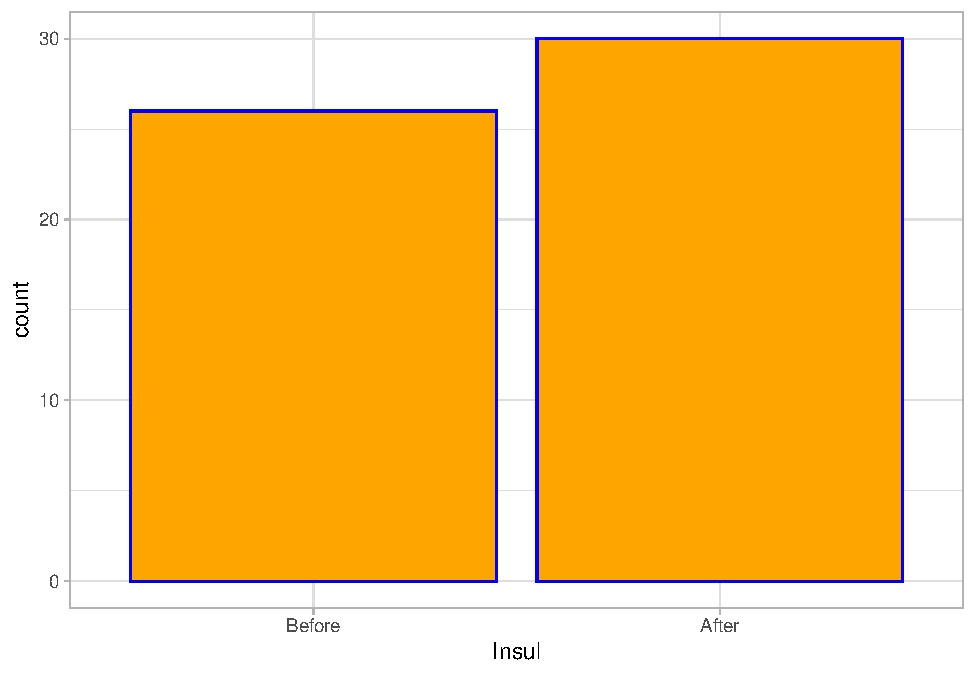
\includegraphics{Chapter-5-Interactive-Notebook-for-Instructors_files/figure-latex/unnamed-chunk-15-1.pdf}

We can now compute any probability we wish from this empirical
distribution. Let us compute the probability that the number of heads
will be less than or equal to 20. Notice that our vector \texttt{s1}
contains the outcomes from 10000 samples. We simply need to count how
many of them satisfy the condition to get our probability.

\begin{Shaded}
\begin{Highlighting}[]
\FunctionTok{length}\NormalTok{(s1[s1}\SpecialCharTok{\textless{}=}\DecValTok{20}\NormalTok{]) }\SpecialCharTok{/}\NormalTok{ (}\FunctionTok{length}\NormalTok{(s1))}
\end{Highlighting}
\end{Shaded}

\begin{verbatim}
## [1] 0.1044
\end{verbatim}

Let us compute the probability of getting 15 or more heads.

\begin{Shaded}
\begin{Highlighting}[]
\FunctionTok{length}\NormalTok{(s1[s1}\SpecialCharTok{\textgreater{}=}\DecValTok{15}\NormalTok{]) }\SpecialCharTok{/}\NormalTok{ (}\FunctionTok{length}\NormalTok{(s1))}
\end{Highlighting}
\end{Shaded}

\begin{verbatim}
## [1] 0.9983
\end{verbatim}

Now let us try something a bit more complicated. We want to repeatedly
keep adding the numbers we get from each roll. The outcome of interest
is the number of times you have to roll the die until you get a sum of
35. The domain here is between 6 and 35, because the minimum number of
rolls needed to obtain a sum of 35 is 6, and the maximum is 35.

\begin{Shaded}
\begin{Highlighting}[]
\NormalTok{diedomain }\OtherTok{=} \FunctionTok{seq}\NormalTok{(}\DecValTok{1}\NormalTok{,}\DecValTok{6}\NormalTok{)}
\NormalTok{dieprob }\OtherTok{=} \FunctionTok{rep}\NormalTok{(}\DecValTok{1}\SpecialCharTok{/}\DecValTok{6}\NormalTok{,}\DecValTok{6}\NormalTok{)}

\NormalTok{v1 }\OtherTok{=} \FunctionTok{sample}\NormalTok{(}\AttributeTok{x =}\NormalTok{ diedomain, }\AttributeTok{size =} \DecValTok{35}\NormalTok{, }\AttributeTok{replace =}\NormalTok{ T, }\AttributeTok{prob =}\NormalTok{ dieprob)}
\NormalTok{c1 }\OtherTok{=} \FunctionTok{cumsum}\NormalTok{(v1)}
\FunctionTok{which}\NormalTok{(c1 }\SpecialCharTok{\textgreater{}} \DecValTok{35}\NormalTok{)[}\DecValTok{1}\NormalTok{]}
\end{Highlighting}
\end{Shaded}

\begin{verbatim}
## [1] 11
\end{verbatim}

There are two functions we used here. The first is \texttt{cumsum()},
which creates a vector whose ith element is the sum from x{[}1{]} to
x{[}i{]}. The second is \texttt{which(x\textgreater{}c)}, which gives
you the index of all the elements of vector x which are greater than the
number c.~We want the first time we see a number greater than 35.
Therefore, we used \texttt{which(c1\ \textgreater{}\ 35){[}1{]}}. Now,
let us put this into a function.

\begin{Shaded}
\begin{Highlighting}[]
\NormalTok{f2 }\OtherTok{=} \ControlFlowTok{function}\NormalTok{()\{}
\NormalTok{  v1 }\OtherTok{=} \FunctionTok{sample}\NormalTok{(}\AttributeTok{x =}\NormalTok{ diedomain, }\AttributeTok{size =} \DecValTok{35}\NormalTok{, }\AttributeTok{replace =}\NormalTok{ T, }\AttributeTok{prob =}\NormalTok{ dieprob)}
\NormalTok{c1 }\OtherTok{=} \FunctionTok{cumsum}\NormalTok{(v1)}
\FunctionTok{which}\NormalTok{(c1 }\SpecialCharTok{\textgreater{}} \DecValTok{35}\NormalTok{)[}\DecValTok{1}\NormalTok{]}
\NormalTok{\}}
\end{Highlighting}
\end{Shaded}

Let us replicate to create the empirical distribution.

\begin{Shaded}
\begin{Highlighting}[]
\NormalTok{s2 }\OtherTok{=} \FunctionTok{replicate}\NormalTok{(}\AttributeTok{n =} \DecValTok{10000}\NormalTok{, }\FunctionTok{f2}\NormalTok{())}
\NormalTok{edf2 }\OtherTok{=} \FunctionTok{prop.table}\NormalTok{(}\FunctionTok{table}\NormalTok{(s2))}
\NormalTok{edf2}
\end{Highlighting}
\end{Shaded}

\begin{verbatim}
## s2
##      7      8      9     10     11     12     13     14     15     16     17 
## 0.0050 0.0576 0.1631 0.2460 0.2297 0.1556 0.0855 0.0373 0.0143 0.0047 0.0012
\end{verbatim}

\begin{Shaded}
\begin{Highlighting}[]
\FunctionTok{plot}\NormalTok{(edf2, }\AttributeTok{type =} \StringTok{"h"}\NormalTok{)}
\end{Highlighting}
\end{Shaded}

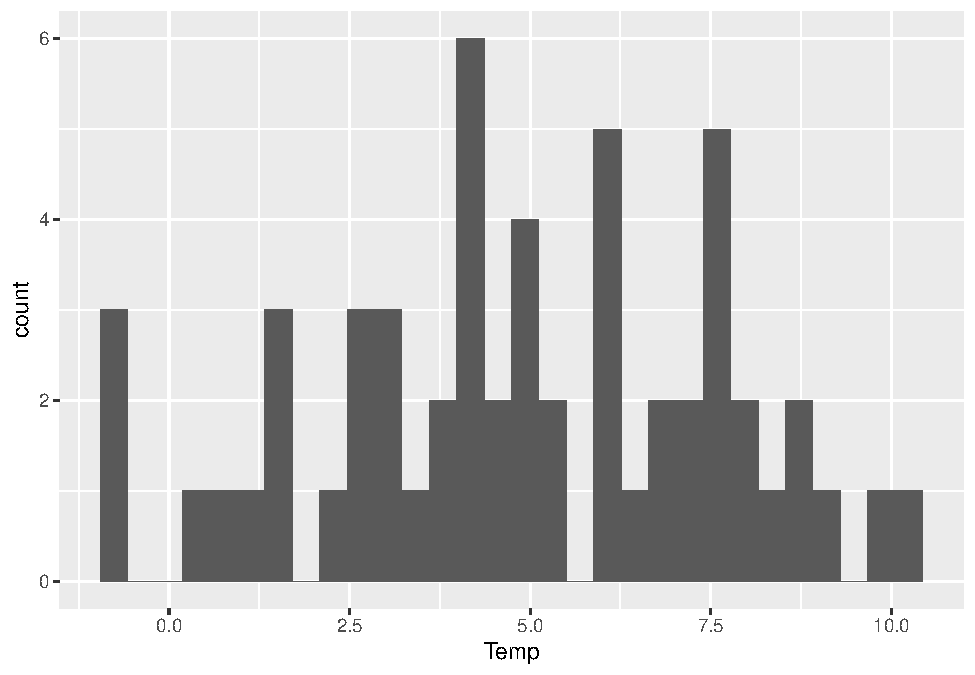
\includegraphics{Chapter-5-Interactive-Notebook-for-Instructors_files/figure-latex/unnamed-chunk-20-1.pdf}

From the plot we see the high probability events are 10 and 11 rolls of
the die.

What is the probability that we will hit 35 in less than or equal to 8
rolls?

\begin{Shaded}
\begin{Highlighting}[]
\FunctionTok{length}\NormalTok{(s2[s2}\SpecialCharTok{\textless{}=}\DecValTok{8}\NormalTok{])}\SpecialCharTok{/}\NormalTok{(}\FunctionTok{length}\NormalTok{(s2))}
\end{Highlighting}
\end{Shaded}

\begin{verbatim}
## [1] 0.0626
\end{verbatim}

Suppose a drug manufacturer guarantees that a particular drug has a .6
probability of working. If the drug was administered to 300 patients, we
want to compute the probability that no more that 160 patients improved
after taking the drug. This example is similar to the previous coin toss
example. However, this time, the number of tosses and the success
probability are different. We will create a more general function where
we can specify the number of trials and the success probability as
inputs to the function. These are the \textbf{parameters} of the
distribution. The following code creates the empirical distribution
function.

\begin{Shaded}
\begin{Highlighting}[]
\NormalTok{drugdomain }\OtherTok{=} \FunctionTok{c}\NormalTok{(}\DecValTok{0}\NormalTok{,}\DecValTok{1}\NormalTok{)}
\NormalTok{f3 }\OtherTok{=} \ControlFlowTok{function}\NormalTok{(sz, successprob)\{}
\NormalTok{  drugprob }\OtherTok{=} \FunctionTok{c}\NormalTok{(}\DecValTok{1}\SpecialCharTok{{-}}\NormalTok{successprob, successprob)}
\NormalTok{  v2 }\OtherTok{=} \FunctionTok{sample}\NormalTok{(}\AttributeTok{x =}\NormalTok{ drugdomain, }\AttributeTok{size =}\NormalTok{ sz, }\AttributeTok{replace =}\NormalTok{ T, }\AttributeTok{prob =}\NormalTok{ drugprob)}
\NormalTok{  s3 }\OtherTok{=} \FunctionTok{sum}\NormalTok{(v2)}
  \FunctionTok{return}\NormalTok{(s3)}
\NormalTok{\}}

\NormalTok{s4 }\OtherTok{=} \FunctionTok{replicate}\NormalTok{(}\AttributeTok{n =} \DecValTok{100000}\NormalTok{, }\FunctionTok{f3}\NormalTok{(}\DecValTok{300}\NormalTok{,.}\DecValTok{6}\NormalTok{))}
\NormalTok{edf3 }\OtherTok{=} \FunctionTok{prop.table}\NormalTok{(}\FunctionTok{table}\NormalTok{(s4))}
\FunctionTok{plot}\NormalTok{(edf3, }\AttributeTok{type =} \StringTok{"h"}\NormalTok{)}
\end{Highlighting}
\end{Shaded}

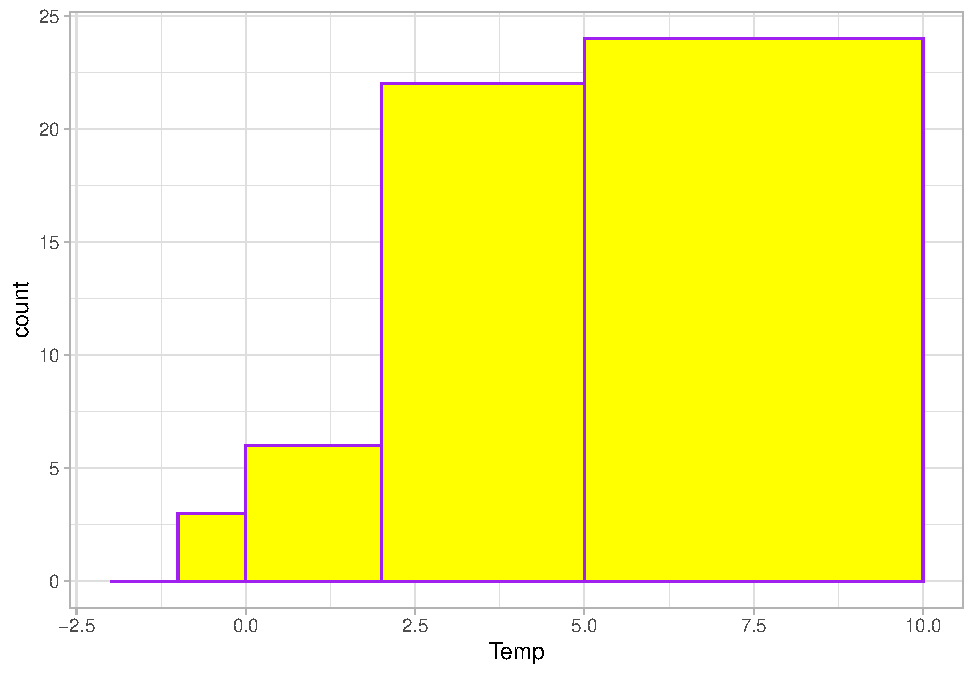
\includegraphics{Chapter-5-Interactive-Notebook-for-Instructors_files/figure-latex/unnamed-chunk-22-1.pdf}

Now we can compute the probability that no more than 160 patients are
cured.

\begin{Shaded}
\begin{Highlighting}[]
\FunctionTok{length}\NormalTok{(s4[s4}\SpecialCharTok{\textless{}=}\DecValTok{160}\NormalTok{])}\SpecialCharTok{/}\FunctionTok{length}\NormalTok{(s4)}
\end{Highlighting}
\end{Shaded}

\begin{verbatim}
## [1] 0.01173
\end{verbatim}

The probability is very small.

Let us think about the following: suppose you know that a medical
facility administered the drug to 300 patients and no more than 160
patients actually improved after taking the drug. What can we say about
this situation?

\begin{enumerate}
\def\labelenumi{\arabic{enumi}.}
\item
  The probability of no more than 160 patients getting better is quite
  small. Even though this is unlikely, it is not impossible.This could
  just be bad luck. For example, you could toss a fair coin ten times
  and get no heads. The probability is very small but it's not zero. If
  I am another medical facility, how would I process this information?
  To rule out the possibility that it was just bad luck, perhaps I would
  want to see more evidence. This can come from procuring a larger
  sample size.
\item
  If you believe the sample size is big enough as it is, then you would
  not attribute the outcome to just bad luck. You will begin to question
  the claims made by the drug manufacturer. Perhaps their claim that the
  drug is effective 60\% of the time is not true. This is the core idea
  behind \textbf{hypothesis testing}. In this case, the drug
  manufacturer's claim of 60\% success constitutes the null hypothesis.
  The sample data allows use to either reject the null hypothesis or not
  reject the null hypothesis. Clearly, in this case we would reject the
  null hypothesis as the probability we computed was very small. We will
  expand on this concept later.
\end{enumerate}

For now, just note that the null hypothesis describes the population,
and the population is described by a distribution. More on this later.

\hypertarget{mean-and-variance-of-a-distribution}{%
\section{Mean and Variance of a
Distribution}\label{mean-and-variance-of-a-distribution}}

As we described before, a discrete distribution is defined by a support,
which is the set of all possible outcomes, and by the corresponding
probability of each outcome. Let \texttt{x\_1,...x\_N} denote the
possible outcomes. Let \texttt{P(x\_i)} denote the probability of
outcome \texttt{x\_i}. The mean and variance are defined as:

\[\mu=\sum_{i = 1}^{N} x_i P(x_i)\]

\[\sigma^2 = \sum_{i = 1}^{N} (x_i - \mu)^2P(x_i)\]

Let us compute the mean and variance of a distribution.

\begin{Shaded}
\begin{Highlighting}[]
\NormalTok{ddomain }\OtherTok{=} \FunctionTok{seq}\NormalTok{(}\DecValTok{1}\NormalTok{,}\DecValTok{4}\NormalTok{)}
\NormalTok{dprob }\OtherTok{=} \FunctionTok{c}\NormalTok{(.}\DecValTok{7}\NormalTok{,.}\DecValTok{1}\NormalTok{,.}\DecValTok{1}\NormalTok{,.}\DecValTok{1}\NormalTok{)}
\NormalTok{meandistribution }\OtherTok{=} \FunctionTok{sum}\NormalTok{(ddomain }\SpecialCharTok{*}\NormalTok{ dprob)}
\NormalTok{meandistribution}
\end{Highlighting}
\end{Shaded}

\begin{verbatim}
## [1] 1.6
\end{verbatim}

\begin{Shaded}
\begin{Highlighting}[]
\NormalTok{vardistribution }\OtherTok{=} \FunctionTok{sum}\NormalTok{((dprob)}\SpecialCharTok{*}\NormalTok{(ddomain}\SpecialCharTok{{-}}\NormalTok{meandistribution)}\SpecialCharTok{\^{}}\DecValTok{2}\NormalTok{)}
\NormalTok{vardistribution}
\end{Highlighting}
\end{Shaded}

\begin{verbatim}
## [1] 1.04
\end{verbatim}

Let us summarize what we know about distributions.

\begin{enumerate}
\def\labelenumi{\arabic{enumi}.}
\tightlist
\item
  The distribution describes all possible outcomes and the corresponding
  probability for each outcome. Each distribution has its support, which
  describes the possible outcome values. For tossing a coin, it is 0 and
  1. For rolling a die, it is 1 to 6.\\
\item
  A distribution is used to describe a population of interest. In this
  sense, it is somewhat of an abstract concept.
\end{enumerate}

\hypertarget{commonly-used-distributions}{%
\section{Commonly Used
Distributions}\label{commonly-used-distributions}}

There are a large number of distributions that have been developed.
These broadly fall into \textbf{discrete} and \textbf{continuous}
distributions. We looked at a number of examples of discrete
distributions thus far. Below are a few common discrete distributions.

\hypertarget{discrete-distributions}{%
\subsection{Discrete Distributions}\label{discrete-distributions}}

\hypertarget{binomial-distribution}{%
\subsubsection{Binomial Distribution}\label{binomial-distribution}}

We in fact looked at a binomial distribution before. The example of
tossing a coin 50 times and a drug delivered to 300 patients. A binomial
distribution has two parameters: the number of trials \(n\), and the
success probability \(\pi\). \(x\) is the random variable that describes
the number of successes in \(n\) trials. The support for this
distribution is \((0,...n)\). The mathematical formulation for a
binomial distribution is:

\[P(x) = \frac{n!}{(x!)(n-x)!}(\pi)^x(1-\pi)^{n-x}\]

The mean and variance of a binomial distribution are:\\
\[mean = n\pi\]\\
\[variance = n\pi(1-\pi)\]

\hypertarget{negative-binomial-distribution}{%
\subsubsection{Negative Binomial
Distribution}\label{negative-binomial-distribution}}

This is in some ways similar to binomial distributions and it has two
parameters: \(r\) and \(\pi\). As before, \(\pi\) is the success
probability. The random variable \(x\) is the number of failures before
the \(r^{th}\) success is observed. Here, the support is between 0 and
\(\infty\), because the number of failures before the \(r^{th}\) success
can be 0 as you can start off with \(r\) consecutive successes, or it
could tend to infinity because the \(r^{th}\) success may never come.
The formula is:

\[P(x) = \binom{x-1}{r-1}(\pi)^r(1-\pi)^r\]

\[mean = \frac{r}{\pi}\]

\[variance = \frac{r(1-\pi)}{\pi^2}\]

\hypertarget{poisson-distribution}{%
\subsubsection{Poisson Distribution}\label{poisson-distribution}}

It is a commonly used distribution for count variables which capture the
number of events or occurrences. It is used to study phenomenon such as
number of claims filed in a year, number of hospital visits in a year,
number of computer crashes in a day, etc. The Poisson distribution has
only one parameter called \$\lambda\$ which describes the expected
number of events. The support is 0 to \(\infty\). The distribution is:

\[P(x) = \frac{e^{-\lambda}\lambda^x}{x!}\]

\[mean = \lambda\]

\[variance = \lambda\]

One interesting thing to note about the Poisson distribution is that the
mean and variance are the same. This is because there is only one
parameter. This can be somewhat restrictive. If you compare this to the
negative binomial distribution, the variance can be bigger or smaller
than the mean in the case of the negative binomial distribution.

\hypertarget{continuous-distributions}{%
\subsection{Continuous Distributions}\label{continuous-distributions}}

Continuous distributions are used for random variables that can take any
value on a continuum. For example, variables like temperature, pressure,
age, salary, are often modeled as continuous variables. Since they are
continuous, there are an infinite number of possible values that a
random variable can take. Due to this fact, a continuous distribution is
depicted through a probability density function \(f(x)\). Let the domain
of the random variable be denoted as \([a,b]\). A probability density
function meets the following criteria:\\
\[\int_{a}^{b} f(x) \; dx = 1\]\\
The mean and variance are defined as:\\
\[\mu = \int_{a}^{b} xf(x) \; dx\]\\
\[\sigma^2 = \int_{a}^{b} (x-\mu)^2f(x) \; dx\]

The cumulative density function is defined as:

\[F(\overline{x}) = \int_{a}^{\overline{x}} f(x) \; dx\]

\(F(\overline{x})\) is the probability that \(x\) is less than or equal
to \(\overline{x}\).

\hypertarget{normal-distribution}{%
\subsubsection{Normal Distribution}\label{normal-distribution}}

The normal or Gaussian distribution is perhaps the most important
distribution in the field of statistics. We will explain why later. Many
naturally occurring events such as heights and weights, and
psychological and educational variables, are typically distributed
approximately normally.

The support for a normal distribution is \([-\infty, \infty]\). The
following describes the normal distribution.

\[f(x) = \frac{1}{\sigma\sqrt(2\pi)} e^{-\frac{1}{2}(\frac{x-\mu}{\sigma})^2}\]

The mean of the standard distribution is \(\mu\) and the variance is
\(\sigma^2\).

If x is normally distributed, we normally write it as
\[x \sim ~N(\mu,\sigma)\]

A standard normal variable \(z\) is defined as

\[ z = \frac{x-\mu}{\sigma}\]

where \[z \sim ~N(0,1)\]

\hypertarget{exponential-distribution}{%
\subsubsection{Exponential
Distribution}\label{exponential-distribution}}

This distribution is used to describe the arrival time of randomly
reoccurring random events. Examples include the time between phone calls
to a call center, time between trucks arriving at an unloading dock, and
time between transactions occurring at an ATM machine. The support for
an exponential distribution is \([0,\infty]\). The probability density
function (pdf) of an exponential distribution and its mean and variance
are:

\[f(x) = \lambda e^{-\lambda x},  x\ge 0,  \lambda>0\]

\[\mu = \frac{1}{\lambda}\] \[\sigma = \frac{1}{\lambda}\]

\hypertarget{uniform-distribution}{%
\subsubsection{Uniform Distribution}\label{uniform-distribution}}

For a uniform distribution in the interval \([a,b]\), the pdf, mean, and
variance are: \[f(x) = \frac{1}{b-a}, a\le x \le b\]
\[\mu = \frac{a+b}{2}\] \[\sigma^2 = \frac{(b-a)^2}{12}\]

\hypertarget{working-with-distributions-in-r}{%
\section{Working With Distributions in
R}\label{working-with-distributions-in-r}}

R provides easy ways to work with various distributions (see the short
reference card). For a given distribution (\textbf{dist}), you can get a
variety of information in R. We precede the distribution name with the
letters \textbf{r} (for random values from the distribution), \textbf{d}
(probability or density value), \textbf{p} (cumulative probability), or
\textbf{q} (value of quantile). Check the R reference card for a list of
common distribution functions.

Recall the drug example with 300 trials and a success rate of .6. The
probability of having no more than 160 cured patients was 0.0116. Let us
do this using the above.

\begin{Shaded}
\begin{Highlighting}[]
\FunctionTok{pbinom}\NormalTok{(}\DecValTok{160}\NormalTok{,}\DecValTok{300}\NormalTok{,.}\DecValTok{6}\NormalTok{)}
\end{Highlighting}
\end{Shaded}

\begin{verbatim}
## [1] 0.01118
\end{verbatim}

As you can see, the answers are very close.

Suppose you want to create 20 random variables from \(N(6,3)\).

\begin{Shaded}
\begin{Highlighting}[]
\FunctionTok{rnorm}\NormalTok{(}\DecValTok{20}\NormalTok{,}\AttributeTok{mean =} \DecValTok{6}\NormalTok{, }\AttributeTok{sd =} \DecValTok{3}\NormalTok{)}
\end{Highlighting}
\end{Shaded}

\begin{verbatim}
##  [1]  8.189  8.049  2.662 -3.284  8.600  8.061  9.971  9.661  6.769  7.107
## [11]  4.469  5.050  5.619  5.138 11.260  4.629 10.242  7.941  6.054 11.535
\end{verbatim}

Let us plot a normal distribution.

\begin{Shaded}
\begin{Highlighting}[]
\FunctionTok{curve}\NormalTok{(}\FunctionTok{dnorm}\NormalTok{(x,}\AttributeTok{mean=}\DecValTok{10}\NormalTok{, }\AttributeTok{sd =} \DecValTok{5}\NormalTok{),}\SpecialCharTok{{-}}\DecValTok{5}\NormalTok{, }\DecValTok{30}\NormalTok{)}
\end{Highlighting}
\end{Shaded}

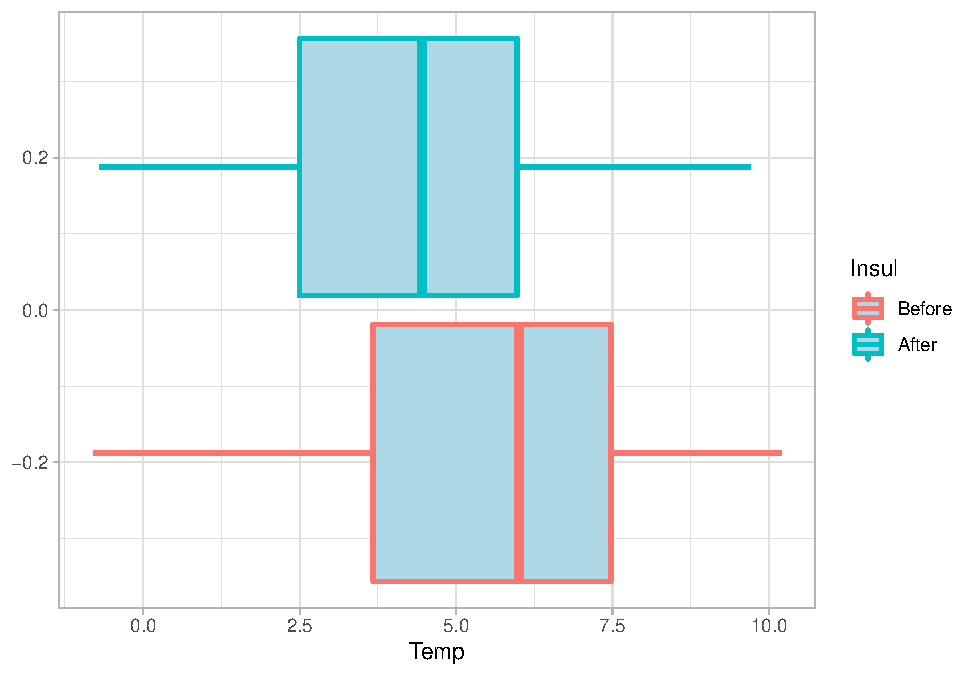
\includegraphics{Chapter-5-Interactive-Notebook-for-Instructors_files/figure-latex/unnamed-chunk-27-1.pdf}

Another way to plot this is to create random numbers from the
distribution and plot the density.

\begin{Shaded}
\begin{Highlighting}[]
\NormalTok{x }\OtherTok{=} \FunctionTok{rnorm}\NormalTok{(}\DecValTok{1000}\NormalTok{,}\AttributeTok{mean =} \DecValTok{10}\NormalTok{, }\AttributeTok{sd =} \DecValTok{5}\NormalTok{)}
\FunctionTok{plot}\NormalTok{(}\FunctionTok{density}\NormalTok{(x))}
\end{Highlighting}
\end{Shaded}

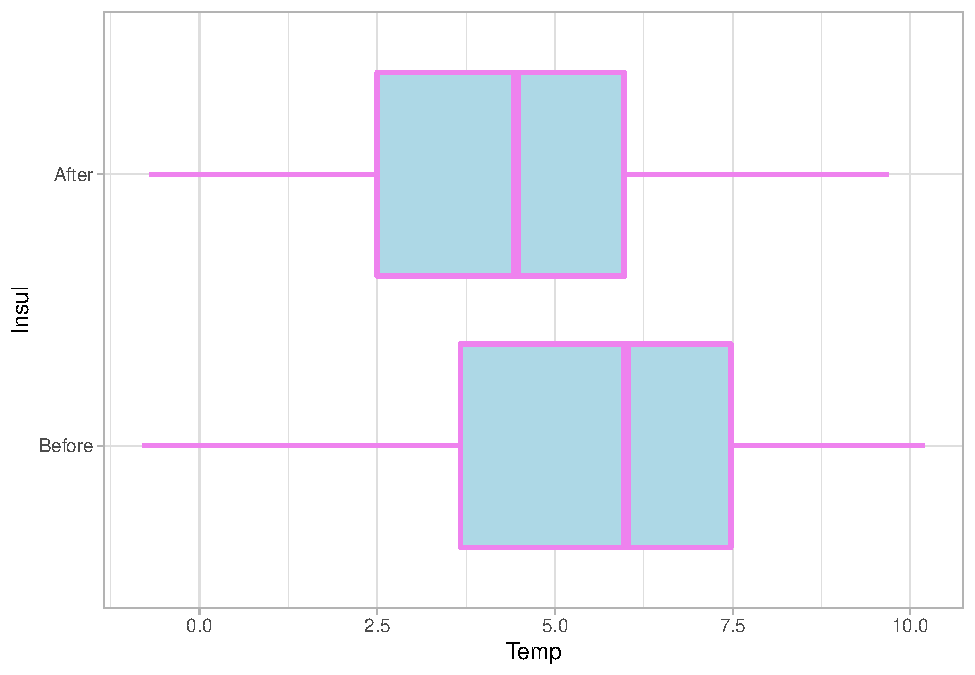
\includegraphics{Chapter-5-Interactive-Notebook-for-Instructors_files/figure-latex/unnamed-chunk-28-1.pdf}

Let us see what an exponential function looks like.

\begin{Shaded}
\begin{Highlighting}[]
\FunctionTok{curve}\NormalTok{(}\FunctionTok{dexp}\NormalTok{(x,}\AttributeTok{rate =} \DecValTok{1}\NormalTok{), }\DecValTok{0}\NormalTok{, }\DecValTok{10}\NormalTok{)}
\FunctionTok{curve}\NormalTok{(}\FunctionTok{dexp}\NormalTok{(x,}\AttributeTok{rate =} \DecValTok{1}\SpecialCharTok{/}\DecValTok{2}\NormalTok{), }\DecValTok{0}\NormalTok{, }\DecValTok{10}\NormalTok{,}\AttributeTok{add =}\NormalTok{ T, }\AttributeTok{col =} \StringTok{"blue"}\NormalTok{)}
\FunctionTok{curve}\NormalTok{(}\FunctionTok{dexp}\NormalTok{(x,}\AttributeTok{rate =} \DecValTok{1}\SpecialCharTok{/}\DecValTok{10}\NormalTok{), }\DecValTok{0}\NormalTok{, }\DecValTok{10}\NormalTok{, }\AttributeTok{add =}\NormalTok{ T, }\AttributeTok{col =} \StringTok{"purple"}\NormalTok{)}
\end{Highlighting}
\end{Shaded}

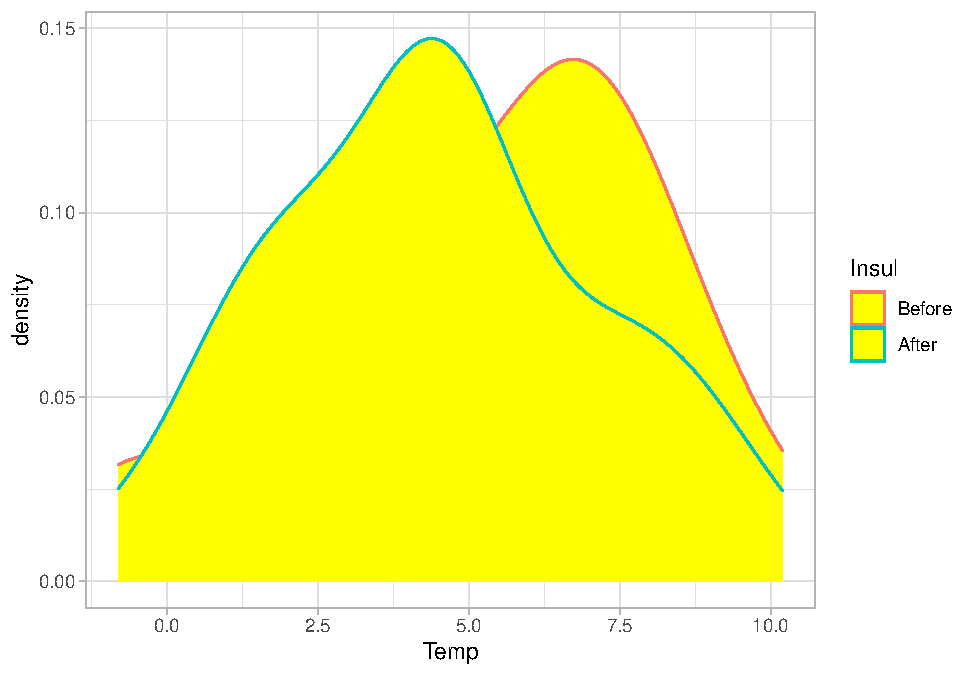
\includegraphics{Chapter-5-Interactive-Notebook-for-Instructors_files/figure-latex/unnamed-chunk-29-1.pdf}

Let us say you want to get the \(75^{th}\) percentile value.

\begin{Shaded}
\begin{Highlighting}[]
\FunctionTok{qexp}\NormalTok{(.}\DecValTok{75}\NormalTok{, }\AttributeTok{rate =} \DecValTok{1}\SpecialCharTok{/}\DecValTok{2}\NormalTok{)}
\end{Highlighting}
\end{Shaded}

\begin{verbatim}
## [1] 2.773
\end{verbatim}

\end{document}
